\documentclass[notes,serif]{beamer}
\usepackage{graphicx}
\usepackage{url}
\usepackage{clrscode}

% You should run 'pdflatex' TWICE, because of TOC issues.

\mode<presentation>
{
  % A tip: pick a theme you like first, and THEN modify the color theme, and then add math content.
  % Warsaw is the theme selected by default in Beamer's installation sample files.
 
  \usetheme{Warsaw}
  
  \usecolortheme{default}

%  \setbeamercovered{transparent} % or whatever (possibly just delete it)
  \setbeamercovered{invisible} % or whatever (possibly just delete it)
  % To change behavior of \uncover from graying out to totally invisible, can change \setbeamercovered to invisible instead of transparent. apparently there are also 'dynamic' modes that make the amount of graying depend on how long it'll take until the thing is uncovered.
}


% Get rid of nav bar
\beamertemplatenavigationsymbolsempty

% Insert frame number at bottom of the page.
\usefoottemplate{\hfil\tiny{\color{black!90}\insertframenumber}}

\usepackage[english]{babel}
\usepackage[latin1]{inputenc}

\usepackage{times}
\usepackage[T1]{fontenc}

\title{Design and Analysis of Algorithms}
\subtitle{Lecture 3---Heapsort}

\author{Lei Wang}

\institute{Dalian University of Technology}

%\date{Date}

\subject{Talks}

\def\defn#1{{\color{red} #1}}

\begin{document}

\begin{frame}
  \titlepage
\end{frame}

\begin{frame}
  \frametitle{Probabilistic Analysis and Randomized Algorithms}
  \tableofcontents
\end{frame}

\section{Overview}
\subsection{Goals}

\begin{frame}
\frametitle{Heapsort}
\begin{itemize}
    \item $O(n \text{lg} n)$ worst case---like merge sort.
    \item Sorts in place---like insertion sort.
    \item Combines the best of both algorithms.
\end{itemize}
To understand heapsort, we'll cover heaps and heap operations, and then we'll take a look at priority queues.

\end{frame}

\section{Heaps}

\subsection{Heap data structure}

\begin{frame}
  \frametitle{Heap data structure}
  \begin{block}{\bf Heap as a tree:}
  Heap $A$ (not garbage-collected storage) is a nearly complete binary tree.
      \begin{itemize}
        \item {\bf \em Height} of node = \# of edges on a longest simple path from the node down to a leaf.
        \item {\bf \em Height} of heap = height of root = $\Theta (\text{lg} n)$. 
      \end{itemize}
  \end{block}
      
  \begin{exampleblock}{{\bf Heap as a array:} A heap can be stored as an array $A$.}
    \begin{itemize}
      \item Root of tree is $A[1]$. 
      \item Parent of $A[i ] = A[	i/2]$. 
      \item Left child of $A[i ] = A[2i ]$.
      \item Right child of $A[i ] = A[2i + 1]$.
      \item Computing is fast with binary representation implementation.
    \end{itemize}
  \end{exampleblock}
\end{frame}

\begin{frame}
  \frametitle{Heap data structure (cont.)}
  \begin{exampleblock}{\bf Heap property:}
      \begin{itemize}
        \item For max-heaps (largest element at root), {\bf \em max-heap property}: for all nodes $i$,
excluding the root, $A[\textsc{Parent}(i)] \ge A[i]$.
        \item For min-heaps (smallest element at root), {\bf \em min-heap property}: for all nodes $i$,
excluding the root, $A[\textsc{Parent}(i )] \le A[i]$.
      \end{itemize}
  \end{exampleblock}

    By induction and transitivity of $\le$, the max-heap property guarantees that the maximum element of a max-heap is {\bf at the root}.  Similar argument for min-heaps.
\end{frame}

\begin{frame}
%\begin{columns}
%  \column{0.7\textwidth}
  \begin{block}{}
    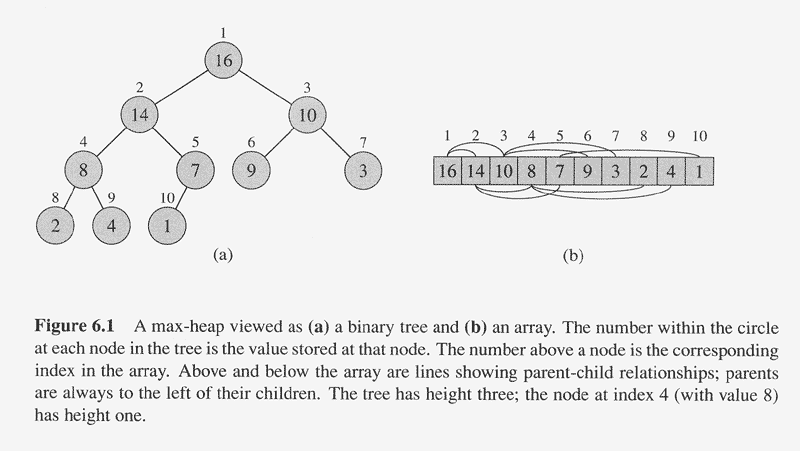
\includegraphics[height=6.1cm]{06-fig-max-heap}
  \end{block}
%\end{columns}
\end{frame}

\begin{frame}
\frametitle{Maintaining the heap property}
  \textsc{Max-Heapify} is important for manipulating max-heaps---to maintain the max-heap property.
  \begin{block}{}
    \begin{itemize}
      {\small
      \item Before \textsc{Max-Heapify}, $A[i]$ may be smaller than its children.
      \item Assume left and right subtrees of $i$ are max-heaps.
      \item After \textsc{Max-Heapify}, subtree rooted at $i$ is a max-heap.
      }
    \end{itemize}
  \end{block}
\begin{columns}
  \column{0.5\textwidth}
  \begin{block}{\textsc{\small Max-Heapify}}
    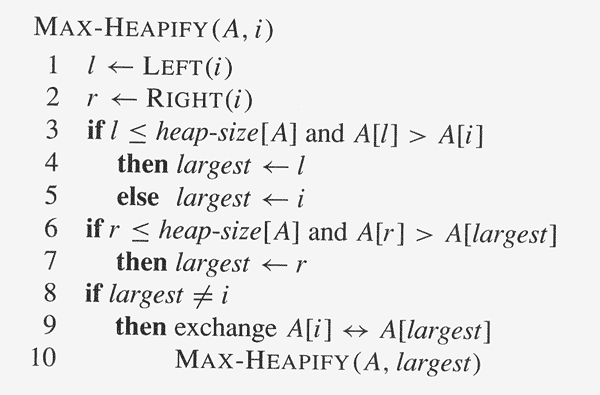
\includegraphics[height=3.5cm]{06-max_heapify}
  \end{block}

  \column{0.5\textwidth}
  \begin{block}{\small The way \textsc{Max-Heapify} works}
  { \small 
  \begin{itemize}
    \item Compare $A[i]$, $A[\textsc{Left}(i)]$, and $A[\textsc{Right}(i )]$.
    \item If necessary, swap $A[i]$ with the larger of the two children to preserve heap property.
    \item Continue until subtree rooted at $i$ is max-heap.
  \end{itemize}
  }
  \end{block}
\end{columns}
\end{frame}

\begin{frame}
\begin{columns}
\column{0.8\textwidth}
  \begin{block}{}
    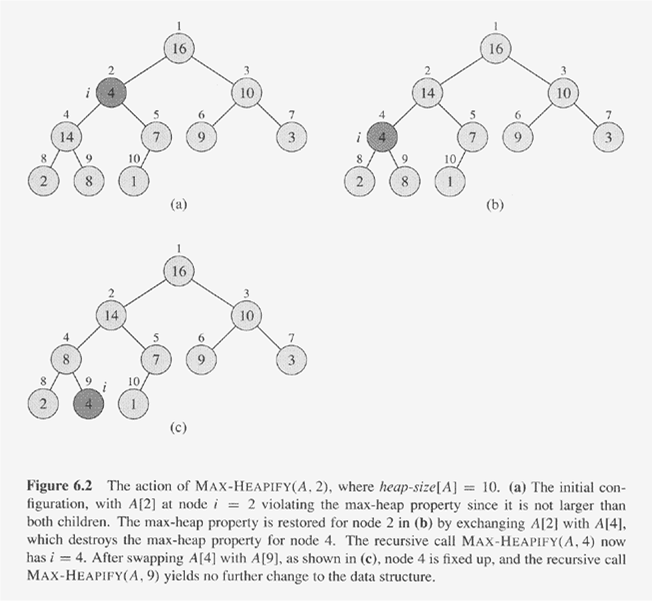
\includegraphics[height=8cm]{06-fig-max_heapify}
  \end{block}
\end{columns}
\end{frame}

\subsection{Building a heap}
\begin{frame}
  \frametitle{Building a heap}
  \begin{block}{\textsc{\small Build-Max-Heap}}
    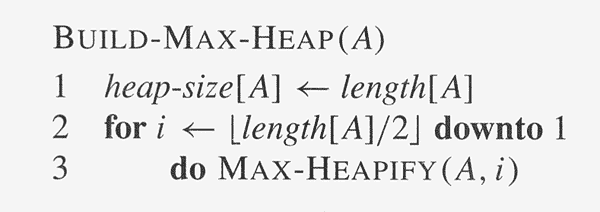
\includegraphics[height=2.5cm]{06-build_max_heap}
  \end{block}
  
  \begin{block}{}
  \begin{itemize}
    \item {\bf \em Simple bound:} $O(n)$ calls to \textsc{Max-Heapify}, each of which takes $O(\text{lg} n)$ time $ \Rightarrow O(n \text{lg} n)$.
  \end{itemize}
  \end{block}
\end{frame}

\begin{frame}
\begin{columns}
  \column{0.68\textwidth}
  \begin{block}{}
    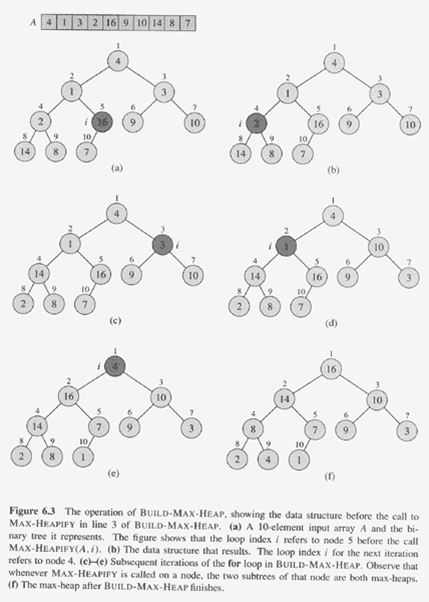
\includegraphics[height=10cm]{06-fig-build_max_heap}
  \end{block}
\end{columns}
\end{frame}

\section{The Heapsort Algorithm}
\subsection{The Heapsort Algorithm}

\begin{frame}
  \frametitle{The Heapsort Algorithm}
  \begin{block}{}
  {\small
  \begin{itemize}
    \item Builds a max-heap from the array. 
    \item Starting with the root, the algorithm places the maximum element into the correct place in the array by swapping it with the last array element.
    \item ``Discard'' this last node by decreasing the heap size, and calling \textsc{Max-Heapify} on the new (possibly incorrectly-placed) root.
    \item Repeat this ``discarding'' process until only one node remains.
  \end{itemize}
  }
  \end{block}

\begin{columns}
  \column{0.6\textwidth}
  \begin{block}{}
    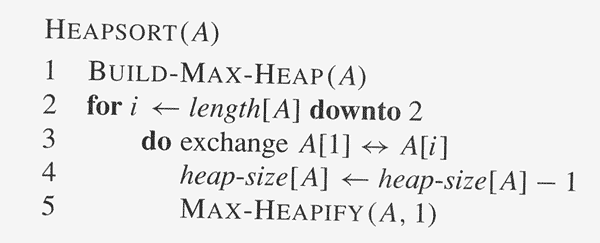
\includegraphics[height=2.5cm]{06-heapsort}
  \end{block}
  
  \column{0.4\textwidth}
  \begin{block}{}
  {\scriptsize
  {\bf \em Analysis:}
  \begin{itemize}
    \item \textsc{Build-Max-Heap}: $O(n)$
    \item for loop: $n-1$ times
    \item exchange elements: $O(1)$
    \item \textsc{Max-Heapify}: $O(\text{lg} n)$
  \end{itemize}
  Total time: $O(n \text{lg} n)$.
  }
  \end{block}
\end{columns}
\end{frame}

\begin{frame}
\begin{columns}
  \column{0.7\textwidth}
  \begin{block}{}
    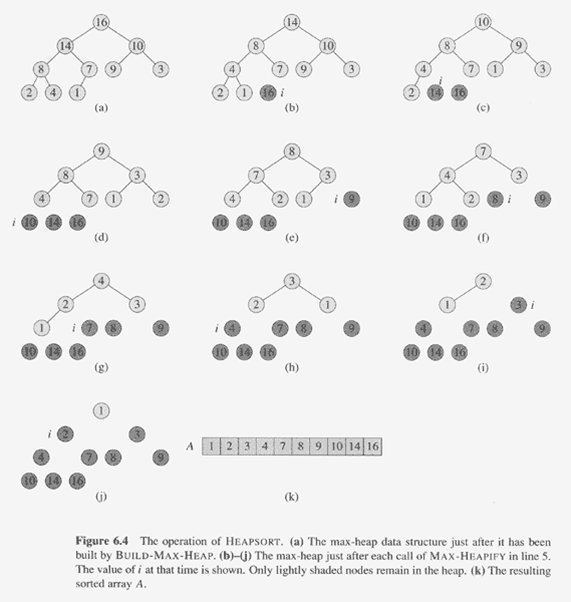
\includegraphics[height=8cm]{06-fig-heapsort}
  \end{block}
\end{columns}
\end{frame}

\section{Heap Implementation of Priority Queue}
\subsection{Priority queue}
\begin{frame}
  \frametitle{Priority queue}
  \begin{itemize}
    \item Maintains a dynamic set $S$ of elements.
    \item Each set element has a key---an associated value.
    \item Max-priority queue supports dynamic-set operations:
    \begin{itemize}
      \item $\textsc{Insert}(S, x)$: inserts element $x$ into set $S$.
      \item $\textsc{Maximum}(S)$: returns element of $S$ with largest key.
      \item $\textsc{Extract-Max}(S)$: removes and returns element of $S$ with largest key.
      \item $\textsc{Increase-Key}(S, x, k)$: increases value of element $x$'s key to $k$.  Assume $k \ge x$'s current key value.
      \item Example max-priority queue application: {\bf schedule jobs on shared computer}.
    \end{itemize}
  \end{itemize}
\end{frame}

\end{document} 